\chapter{Power supply system design}
\section{System overview} \label{sec:literature_system}

\begin{figure}[h]
    \centering
    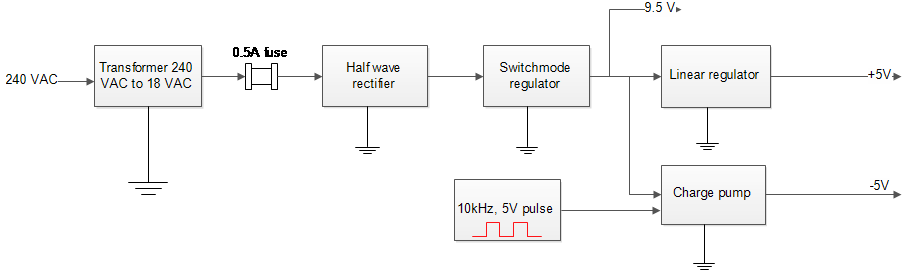
\includegraphics[width = 0.825\linewidth]{Figures/system_overview}
    \caption{System diagram}
    \label{fig:system_diagram}
\end{figure}

\section{Rationale}\label{sec:rationale_system}
The \SI{240}{VAC} to \SI{18}{VAC} transformer was provided for this design, to avoid the risk associated with working directly with the mains supply voltage. As only a half wave rectifier is implemented in the design the AC return can be directly connect to the DC ground. The rectifier provides a positive voltage that is passed through two stages of regulation. 

The switchmode regulator is connected to the rectifier as it is more efficient at higher input voltages \cite{regulators-main}. However,it produces significant noise in its output which is unwanted in this device's application. So, the switchmode is adjusted to give an intermediate voltage that drives a linear regulator to give a \SI{+5}{\volt} supply, and a charge pump scheme to supply \SI{-5}{\volt}.This allows for minimal noise in the \SI{+5}{\volt} rail, and increases the efficiency of the charge pump scheme. 







